Pro parsování dokumentu do AST byl vytvořen vlastní parser. Tvorba parseru se ukázala jako nejnáročnější část realizace.
Pro zjednodušení implementace v sobě parser využívá (rozšířené) regulární výrazy kde je to možno. Jejich použití pak
doplňuje například použitím počítadla pro správné ukončování vnitřních prostředí. Dále je používán zásobník, který
umožnuje sledovat aktuální \textit{scope}.

\begin{sloppypar}
Pro parsování meta-bloků (odsazených YAML bloků) byla využita knihovna yaml. Jedná se o aktivně udržovanou, populární
knihovnu (4 až 12 milionů týdenních stažení z npm \cite{npm} během posledního roku) s permisivní open-source licencí,
která také poskytuje TypeScript \textit{types}.
\end{sloppypar}

Parser korektně parsuje každý jednostránkový validní WooWoo dokument. Nechává ale oproti WooWoo specifikaci větší
volnost v prázdných řádcích mezi bloky, objekty a částmi dokumentu. Dále parser podporuje vnořená vnější prostředí, což
opět WooWoo specifikace \cite{woowoo} nedovoluje (narozdíl od objektů). Parser tedy parsuje i některé dokumenty, které
nejsou zcela validní dle WooWoo specifikace. Direktivy \mintinline{text}{.include} aktuálně podporovány nejsou a parser
je považuje za normální text bez speciálního významu.

Parser podporuje jak novou zkrácenou formu vnitřního prostředí se zavináčem, tak starší zkrácenou formu s tečkou. Je
tomu z důvodu použití starší zkrácené formy ve zdrojích existujících studijních textů.

Každý vrchol výsledného AST dědí z abstraktní třídy \mintinline{text}{ASTNode}. Tato abstraktní třída deklaruje druh
vrcholu, jeho rodiče (může být prázdný, což znamená vrchol stromu), seznam jeho dětí (může být prázdný, což znamená list
stromu), jestli je křehký, počáteční a koncovou pozici ve zdroji (řádek, sloupec a odsazení od počátku souboru) a jeho
meta-data. \mintinline{text}{ASTNode} také definuje funkce pro porovnání dvou vrcholů nebo výpis vrcholu do JSON.

Dále mohou vrcholy implementovat interface \mintinline{text}{ValueASTNode} (který deklaruje hodnotu vrcholu) a
rozšiřovat abstraktní třídu \mintinline{text}{VariableASTNode} (která rozšiřuje abstraktní třídu \mintinline{text}
{ASTNode} a deklaruje variantu vrcholu). Variantou vrcholu je myšlen typ částí dokumentu, objektů a vnějších či
vnitřních prostředí (slovo \mintinline{text}{variant} bylo použito namísto slova \mintinline{text}{type}, protože
\mintinline{text}{type} je dle \cite{ts-docs} v jazyce TypeScript klíčové slovo).

Na obrázku \ref{parsovani-ast} je ilustrován (bez detailů jako pozice vrcholu nebo typ/varianta) AST vzniklý parsováním
zdroje \ref{parsovani-ast-zdroj}.

\begin{figure}\centering
    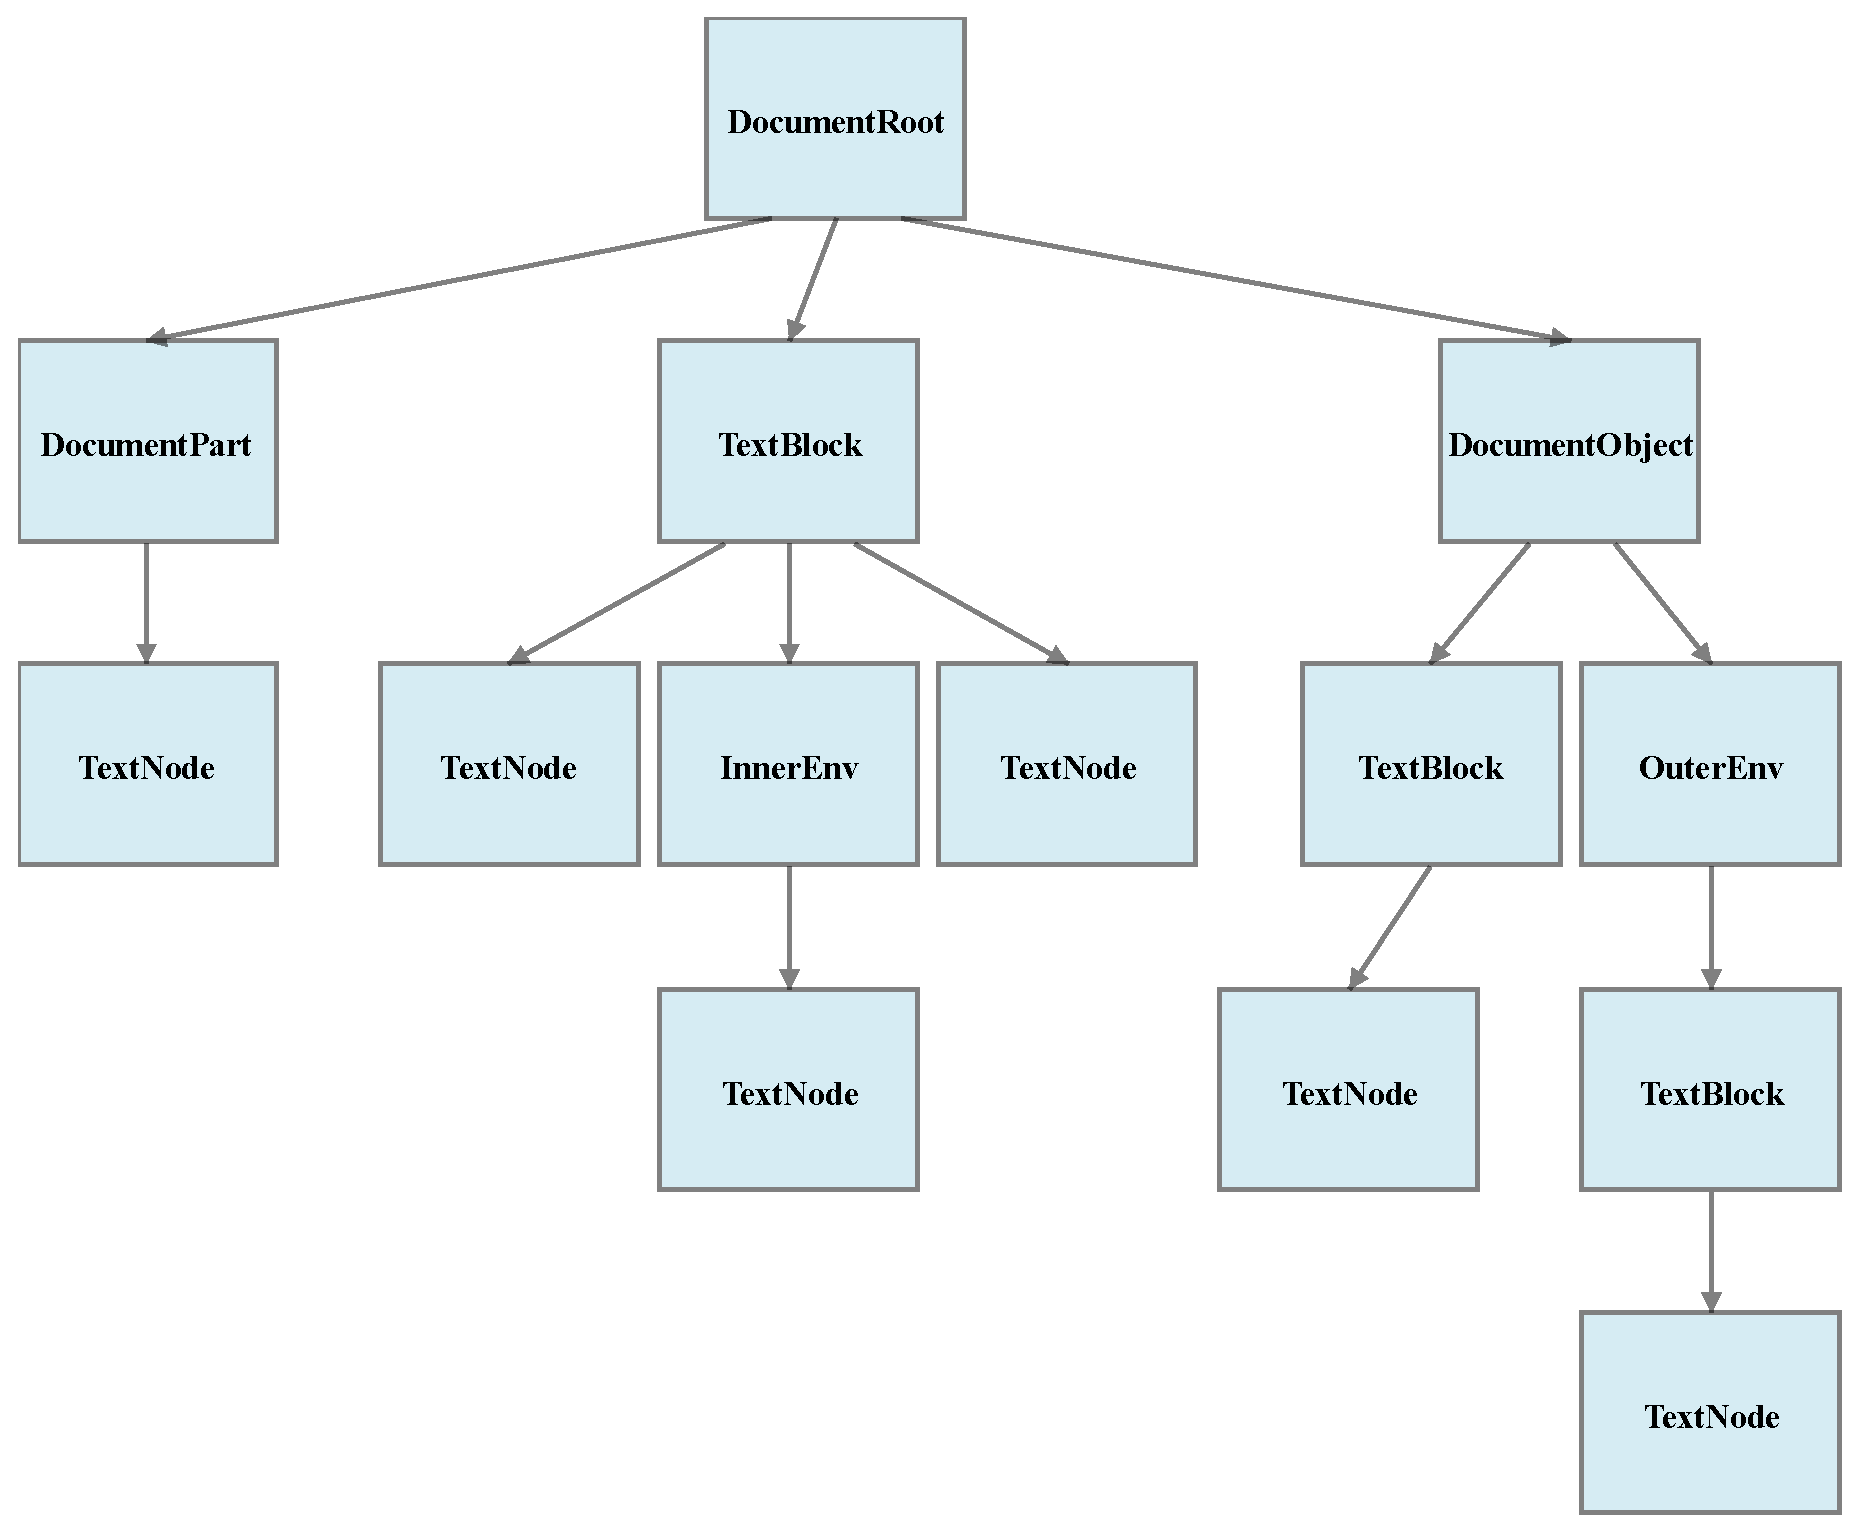
\includegraphics[width=1.0\textwidth]{content/realizace/parsování-ast}
 	\caption[WooWoo AST]{AST vzniklý parsováním WooWoo zdroje~\ref{parsovani-ast-zdroj}}
    \label{parsovani-ast}
\end{figure}

\begin{listing}
    \caption{WooWoo zdroj, jehož AST je ilustrován na obrázku~\ref{parsovani-ast}}
    \label{parsovani-ast-zdroj}
    \begin{minted}[breaklines]{text}
.Chapter Jméno kapitoly
  label: chap-1

text text "text text".emphasize text


.Question:

  text text "text text".emphasize text?

  .solution:

    Řešení
    \end{minted}
\end{listing}
